\documentclass[]{tufte-book}

% ams
\usepackage{amssymb,amsmath}

\usepackage{ifxetex,ifluatex}
\usepackage{fixltx2e} % provides \textsubscript
\ifnum 0\ifxetex 1\fi\ifluatex 1\fi=0 % if pdftex
  \usepackage[T1]{fontenc}
  \usepackage[utf8]{inputenc}
\else % if luatex or xelatex
  \makeatletter
  \@ifpackageloaded{fontspec}{}{\usepackage{fontspec}}
  \makeatother
  \defaultfontfeatures{Ligatures=TeX,Scale=MatchLowercase}
  \makeatletter
  \@ifpackageloaded{soul}{
     \renewcommand\allcapsspacing[1]{{\addfontfeature{LetterSpace=15}#1}}
     \renewcommand\smallcapsspacing[1]{{\addfontfeature{LetterSpace=10}#1}}
   }{}
  \makeatother
\fi

% graphix
\usepackage{graphicx}
\setkeys{Gin}{width=\linewidth,totalheight=\textheight,keepaspectratio}

% booktabs
\usepackage{booktabs}

% url
\usepackage{url}

% hyperref
\usepackage{hyperref}

% units.
\usepackage{units}


\setcounter{secnumdepth}{-1}

% citations
\usepackage{natbib}
\bibliographystyle{plainnat}

% pandoc syntax highlighting

% longtable

% multiplecol
\usepackage{multicol}

% strikeout
\usepackage[normalem]{ulem}

% morefloats
\usepackage{morefloats}


% tightlist macro required by pandoc >= 1.14
\providecommand{\tightlist}{%
  \setlength{\itemsep}{0pt}\setlength{\parskip}{0pt}}

% title / author / date
\title{Re-envisioning a future in scholarly communication}
\author{Chris H.J. Hartgerink}
\date{2017-05-23}


\begin{document}

\maketitle




\textbf{For the 2017 IFLA conference, theme: Being open about open}

\textbf{Made available under a
\href{https://creativecommons.org/publicdomain/zero/1.0/legalcode}{CC 0
public domain dedication}}

\section{Abstract}\label{abstract}

Scholarly communication is in need of disruption. Commodifying knowledge
as is currently done with journals, is not sustainable any longer. An
alternative is the commodification of how information is consumed. By
focusing on the commodification of consumption instead of
commodification of the resource, the problem of access to knowledge can
be resolved in a sustainable manner. Additionally, commodification of
consumption removes several perverse incentives from the scholarly
system that now produces unreliable knowledge. The main tenet underlying
the themes of Open Access, Open Data, Open Science, and replication
initiatives in scholarly communication is sustainability through
transparency of the scholarly process in all facets. The sustainability
of any networked system is threatened by single points of failure (i.e.,
the entire system can be manipulated from one node in the network). The
scholarly process is ridden with such single points of failures at all
stages. Distributing the scholarly communications system would remove
the problems of single points of failure. Distributing and
decentralizing the scholarly communications system is achievable with
newly developed peer-to-peer (p2p) Internet protocols. Alongside
decentralization and distribution of the content, integrity of the
scholarly record can also be reformed to transform sections of a paper
into different, reusable nodes of knowledge. These nodes can be logged
on a blockchain based ledger of which everyone can have a copy. In order
to deposit nodes onto the ledger, the depositor needs to agree that the
contents are licensed CC 0, in order to maximize legal certainty
regarding reuse of the contents. This is key to create a sustainable
eco-system where scholars and companies can cooperate instead of
compete, as we currently do.

\section{Body}\label{body}

Scholarly communication is in (dire) need of disruption. Subscription
costs to scholarly journals are untenable already
\citep[e.g.,][]{harvard-serials-crisis} and will become even more
untenable in the long run with above inflation price-increases
\citep[i.e., serials crisis;][]{serials-crisis}. The current scholarly
incentive system detracts validity instead of adding it
\citep[e.g.,][]{10.1371/journal.pmed.0020124, 10.1371/journal.pmed.0050201}
by promoting behavior that is antithetical to the norms of science
\citep{merton1942, 10.2307/2094423, 10.1525/jer.2007.2.4.3}. For
example, results particular to one researcher instead of universal among
researchers, because results cannot systematically be verified
considering data are rarely shared
\citep{10.1038/nature.2017.21549, 10.1525/collabra.13, 10.1037/0003-066x.61.7.726}
or preserved \citep{10.1016/j.cub.2013.11.014}. Widely publicized
results regularly fail reproducibility tests
\citetext{\citealp[e.g.,][]{10.1126/science.aac4716}; \citealp{10.1038/483531a}; \citealp{10.1038/541269a}; \citealp[but
see also][]{10.1016/j.jesp.2015.10.001}}, in part because published
results are highly pre-selected for unscientific reasons
\citetext{\citealp[e.g., pure novelty of
results,][]{10.1016/j.tree.2013.05.007}; \citealp[easy to assimilate
findings,][]{10.1038/526182a}; \citealp[statistical
significance,][]{10.1126/science.1255484}; \citealp{10.1016/0140-67369190201-Y}}.
These problems are not new but they are also not absolute --- scholars
want to behave in accordance with the scientific norms
\citep{10.1525/jer.2007.2.4.3} but the system seems to encourage us to
do the opposite.

In this perspective piece, I try to radically reimagine the scholarly
communications infrastructure based on the digital tools that are
available to us now, instead of the analog era and its legacies. I
thoroughly believe that the Mertonian norms in science
\citep{merton1942} align perfectly with transparency in science
\citep[see also][]{10.14293/s2199-1006.1.sor-socsci.arysbi.v1} and that
a scholarly communications system can be built on this framework in a
sustainable manner. I invite everyone to criticize these ideas, for only
with diversity of ideas can we truly make progress. Currently, how
scholars operate (i.e., governance) is driven by a few oligopolies
\citep{10.1371/journal.pone.0127502} or the highly pre-selected sample
of tenured professors and policymakers, who mostly stem from the
generation that has created this broken system and have benefited or
still benefit from the current system. As a result, they are likely to
underestimate the need for change in scholarly communications and cannot
be expected to intervene in the necessary ways.

In the last decades, interpersonal communication has changed
tremendously. Not only has it brought much diversity in communication,
so much diversity has come into existence that it has become confusing
(see Figure 1). At the same time, that same diversity has liberated us
by allowing innovative ways to communicate (e.g., social media) or
making available previously difficult to use safety measures easily
accessible to the masses (e.g., encryption). Diversity in
communication-channels has thus spawned new ways of communicating.

\begin{figure}

{\centering 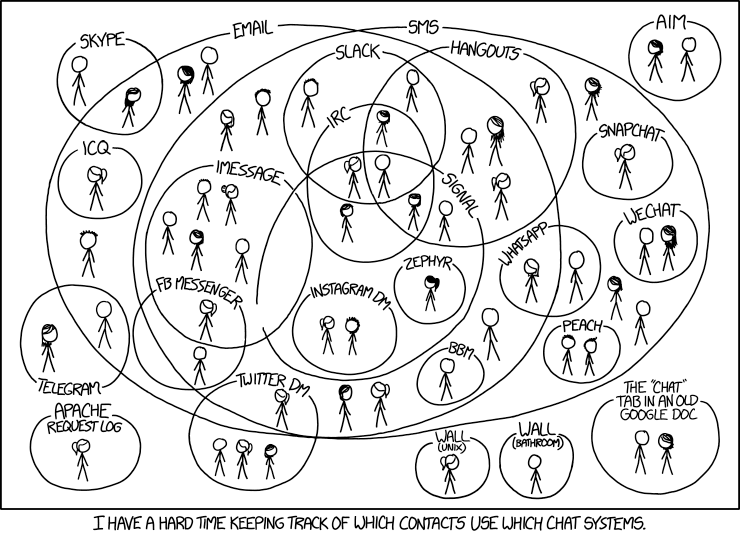
\includegraphics[width=0.6\linewidth]{figs/xkcd_1810-cc-by-nc-2_5} 

}

\caption[_Figure 1._ A comical example of the diversity in communication channels]{_Figure 1._ A comical example of the diversity in communication channels. [Licensed under CC BY-NC 2.5 from xkcd](https://xkcd.com/1810/)}\label{fig:xkcd-1810}
\end{figure}

The current scholarly communications system requires submitting to a
journal that fits all scholarly output into a static, page-by-page, and
paper format without the innovative solutions that are now available.
This bottleneck not only prevents new ways of communicating findings, it
also prevents further encouragement of discussion amongst readers about
the findings. As a result, the current system encourages scholars to
passively consume findings instead of critically evaluating them.

Hence, we are stuck in a paper paradigm, albeit writing digital pages.
Such digital pages radically restrict the way we imagine the
communication of our results. In recent years, options to break free
from this paper paradigm have arisen with tools such as
\href{http://rmarkdown.rstudio.com/}{Rmarkdown} or
\href{https://jupyter.org/}{Jupyter notebooks}. These options allow the
user to include code to dynamically generate figures, tables, or values
in the text. By extension, how data are cleaned and analyzed can also be
included as part of a manuscript for co-authors to verify or readers to
discuss \citep[see also][]{elife-rmd}. Moreover, interactive elements
can be embedded, such as interactive figures, online applications, or
videos.

The scholarly process is much more complicated than can be captured in a
single static and retrospective publication. The previously mentioned
interactive elements enrich a single publication, but multiple moments
of communicating ideas and results maps the empirical cycle onto the
communication process. For example, a quantitative scholar needs to
develop methods to investigate a research question. Feedback from peers
would be valuable at that point. With so called Registered Reports
\citep{10.1016/j.cortex.2012.12.016} a two-staged submission process is
introduced to move away from a single static publication. It allows
selected peers (i.e., peer reviewers) to discuss the contents at an
interim stage. Additionally, this ensures chronology of predictions such
as pre-registrations aim to do \citep{10.1038/s41562-016-0021}, but in a
more natural way. Nonetheless, registered reports, pre-registration, and
data sharing are for the proactive, hence, remain the exception rather
than the norm \citep{10.1371/journal.pbio.1002456}, while these are
already implicitly part of how scholarly research is conducted.
Additionally, researchers create materials, protocols, and other outputs
during the research process, share them with colleagues/advisors, but
this process is not (aptly) sharable in a static publication. If the
scholarly research process has more moments of communication, these
implicit parts are finally able to show themselves.

Additionally, the scholarly process has grown more complicated with the
rise of research tools available and the speed with which alternative
results can be inspected. Point-and-click software has increased the
number of statistical analyses a researcher can do within minutes. This
increased researcher degrees of freedom to present results that are more
in line with previous results, leading to confirmation bias or motivated
reasoning \citep{10.1037/0033-2909.108.3.480}, hence, invalid results
\citep{10.1177/0956797611417632}. Moreover, the development of
technology has created new types of data output that greatly exceed
human comprehension and require algorithms before being able to make
sense of the data (e.g., fMRI data). How a researcher applies all these
tools is essential, but the current scholarly communication system does
not require communication of the details needed to understand what steps
were taken. Lack of direct reproducibility of results
\citep[e.g.,][]{10.1101/056473} therefore is no surprise when we do not
know how data are processed and analyzed. As such, the scholarly process
has become more of a black box than it was before because communication
has not adapted proportionate to the increasing complexity of the
message that needs to be communicated. Increasing complexity and lack of
transparency makes it increasingly difficult to reproduce steps taken,
simply due to an increasing garden of forking paths
\citep{10.1511/2014.111.460}.

Due to the fact that these complexities currently cannot and therefore
are not reported, breaking the reign of the paper paradigm is a
necessity to better represent and understand how scholarly results come
into existence. Static paper publication remains a valid communication
medium and it is not made obsolete when scholarly communications become
truly digitally born and continuous. PDF versions of outputs can still
be produced if a paper format is suitable or desirable. However, it is
easy to imagine videos being embedded for protocols to be easily
clarified (having ``Video X'' alongside ``Figure X'' and ``Table X'',
for example) by origin, to then be replaced by stills when a paper
version is produced. Nonetheless, without shifting the main focus from
paper-based to digital-based scholarly communication, we cannot break
free from the legacies of the paper paradigm. Paper-based communication
includes the legacy of printing research outputs by default, which by
extension includes the idea of subscriptions, purchasing content, and
restricting the flow of information. Copyright is the legacy of the
paper-based age that seems to limit the digital potential of scholarly
outputs. As such, the legacy of a paper-based paradigm with respect to
scholarly communication is that of knowledge commodification.

For scholarly communication, commodifying knowledge as it is currently
done can be seen as a human rights violation.
\href{http://wayback.archive.org/web/20170510094028/http://www.un.org/en/universal-declaration-human-rights/index.html}{The
Universal Declaration of Human Rights (UDHR), Article 27 section 1},
reads as follows

\begin{quote}
Everyone has the right freely to participate in the cultural life of the
community, to enjoy the arts and to share in scientific advancement and
its benefits.
\end{quote}

When knowledge is commodified, it results in decreased participation,
enjoyment, and sharing of scholarly progress. It could therefore be
argued that this is a violation of human rights \citep{udhr}. Moreover,
this is the main legal motivation proposed by Alexandra Elbakyan as to
why \href{http://sci-hub.bz}{Sci-Hub} is not illegal from her point of
view \citep{alexandraelbakyan}. Discussion on the legal correctness of
this argument would be worthwhile to further learn about this. On the
other hand, legal cases on this could result in clarification of whether
unauthorized sharing, which is part of scholarly culture
\citep{10.1038/545145a}, is allowed from a human rights perspective and
whether such sharing would supercede copyright legislation.

Moreover, commodifying knowledge is not the only way to make scholarly
communication sustainable; an alternative is the commodification of how
information is consumed. That is, commodifying the services that serve
the users the content, instead of the content itself. For example, if
all scholarly information is freely available, (not-)for-profit
organizations can compete for users who want to sift through that
information efficiently. If an algorithm is developed that greatly
increases efficiency of finding relevant articles, revenue could be
built with usage fees to that service instead of the content. Such a
market could create competition in information consumption, which is
timely given the information explosion humanity is going through at the
moment. The potential market capitalization of free flow of information
and data is tremendous \citep[e.g., freely reusable public sector
information/data in the U.K. is estimated to provide a market cap of
£590 million - £16 billion; p.~96 of][]{dotecon}. A freely reusable
information resource would provide the infrastructure that encourages
innovation and competition as to how people can discover and consume
that information.

Consequently, by focusing on the commodification of consumption instead
of commodification of the resource, the problem of access to knowledge
can be resolved in a sustainable manner. When the consumption is
commodified, all service providers benefit from creating the largest
pool of resources that is freely available to build their service on. By
extension, it shifts the optimal outcome from not sharing (i.e.,
defecting) to sharing (i.e., cooperating), because it increases the
value of their service. This would create a market that stimulates
access instead of limiting it, while retaining the potential for
revenue.

Additionally, commodification of consumption removes several perverse
incentives from the scholarly system that now produces unreliable
knowledge. For example, innovativeness and surprisingness are criteria
upon which articles are currently selected, where those exact some
properties increase the probability that the finding is false
\citep{10.1371/journal.pmed.0020124}. When the knowledge is commodified,
this makes sense from a business perspective (comparable to news
outlets): readers will buy access more to shocking and astounding
results. However, when consumption is commodified, this whole incentive
is removed and the most valuable resource is the most populated and
diverse one. This would allow much more information to be extracted,
hence, richer services to be built on top of that resource.

The main tenet underlying the themes of Open Access, Open Data, Open
Science, and replication initiatives in scholarly communication is
sustainability through transparency of the scholarly process in all
facets. As I tried to explain in the previous paragraphs, this
sustainability can be achieved by recalibrating the fundamental business
model of the scholarly communications system. In the next section of
this perspective piece, I propose a redesign of the scholarly
communication system that is flexible, decentralized, distributed, and
freely accessible and reusable from the start. Such a system would allow
for more sustainability and diversity in the way we consume, produce,
and access knowledge, which would ultimately benefit everyone who reaps
the benefits of scholarly results.

\section{Sustainable scholarly
communication}\label{sustainable-scholarly-communication}

The sustainability of any networked system is threatened by single
points of failure (i.e., the entire system can be manipulated from one
node in the network). Single points of failure not only make a system
vulnerable to downtime, it also raises the possibility of (malicious)
adjustment of content, or even complete removal of content (among other
things). For example, retracted papers sometimes wholly disappear,
leaving only the retraction notice; this results in a direct and nearly
irreversable adjustment of the scholarly record (from the scholar's
perspective). Due to these single (or few) points of failure, such a
centralized and concentrated infrastructure is easier to disrupt than a
decentralized or distributed one \citep[see
also][]{10.1103/physreve.95.022313}.

The scholarly process is ridden with single- or few points of failures
at all stages. Hence its sustainability is directly threatened. As
mentioned before, communication occurs only once (i.e., at the end);
this could be regarded as a single point of failure for communicating
what the scholars did. If data are not shared or preserved, the scholar
creates a single point of failure in accessing and preserving the data.
When results are published with a closed access publisher, the publisher
becomes the single point of failure for providing access to those
results. For exactly this reason I find it important that scholars
become more transparent about their data, their hypotheses, their
results, and the chronology of their research process; it decreases the
risk of a single point of failure actually failing.

Distributing the scholarly communications system would remove the
problems of single- or few points of failure in access to findings.
Currently, \href{http://www.portico.org/digital-preservation/}{Portico}
and \href{https://clockss.org/clockss/Home}{CLOCKSS} are supposed to
provide access in case the original content is subject to a
\href{https://clockss.org/clockss/FAQ\#How_does_the_CLOCKSS_board_define_a_trigger_event.3F}{``trigger
event''} (e.g., publisher goes out of business). However, this system is
insufficient for wide distribution because content is only selectively
distributed to libraries. Moreover, by its nature ``trigger events'' are
reactive and need governance (indicated by the Centralized LOCKSS
system, i.e., CLOCKSS). That such governance is problematic, is
subscribed by the case that CLOCKSS has previously preserved content
under a more restrictive license than was originally used
(\href{http://wayback.archive.org/web/20170518110938/https://clockss.org/clockss/Tijdschrift_voor_Tijdschriftstudies}{CC
BY-NC-ND for the preserved journal ``Tijdschrift voor
Tijdschriftstudies''}, whereas
\href{http://triggered.stanford.clockss.org/ServeContent?url=https\%3A\%2F\%2Fwww.tijdschriftstudies.nl\%2Farticles\%2F10.18352\%2Fts.340\%2Fprint\%2F}{the
original was CC BY}). In order to make a truly distributed system
sustainable, persistent nodes in the network need to be identified to
store all this information (e.g., libraries), but institutions and
individuals should be able to freely participate in the distributed
network by freely creating temporary or persistent copies for wide and
unlimited distribution of content.

Distributing and decentralizing the scholarly communications system is
achievable with peer-to-peer (p2p) Internet protocols such as
\href{https://datproject.org/}{\texttt{dat}} and
\href{https://ipfs.io/}{\texttt{ipfs}}. Simply put, such p2p networks
securely send information across a network of peers but are resilient to
nodes being removed or adjusted because they operate in a mesh network.
For example, if 20 peers have file X, removing one peer does not affect
the availability of the file X. Only if all 20 are removed from the
network, file X will become unavailable. Vice versa, if more peers on
the network have file X, it is less likely that file X will become
unavailable. As such, this would include unlimited redistribution in the
scholarly communication system by default, instead of limited
redistribution due to copyright as it is now.

Alongside decentralization and distribution of the content as described
in the previous paragraphs, integrity of the scholarly record can also
be reformed to transform sections of a paper into different, reusable
nodes of knowledge. The chronology of the scholarly process can be
ensured by splitting up the paper article as we know it into nodes of
information. The theory section could be a node, from which a hypotheses
node follows, from which a methods node follows, and so on. This would
provide a more true depiction of the scholarly process and facilitate
direct replications (one needs to only take the materials node and
create a new data node), reanalyses (one needs to only take the data
node and create a new results node), etc. Additionally, scholars would
be able to start citing more granularly by referring to specific nodes
instead of entire papers and would not have to write the same theory
section (for example) multiple times for different papers.

These nodes can be logged on a blockchain based ledger (e.g.,
\href{https://github.com/hyperledger/fabric}{Hyperledger}-based) of
which everyone can have a copy. Although explaining the entire operating
principle of the blockchain is beyond the scope of this piece, the
essence is relatively simple. Each entry on the blockchain needs to
satisfy a predefined mathematical rule, which is dependent on the
contents of the previous entry in the ledger, the contents of the new
entry, and a constant to offset the current entry \citep{bitcoin}.
Creating a situation that fullfills that mathematical rule requires
solving for the offset in the new entry to the blockchain, which is
called `mining'. Because the proof of record (i.e., satisfying the
predefined mathematical rule) is dependent on the combination between
the contents of the previous- and current entries (i.e., blocks) and the
offset, the chain is broken when the contents of any entry in that chain
are (unwillingly) changed. Given that each user has a copy of the entire
blockchain, those who have a different chain from the majority of other
users are simply rejected. As such, in order to change the ledger, each
change would have to be re-verified by the majority of the network
(i.e., \textgreater{}50\%) to become verified (for a good introduction
to the blockchain, see
\url{https://www.youtube.com/watch?v=_160oMzblY8}).

Figure 2 shows an example of how the nodes might be incorporated into
such a blockchain based ledger. The idea behind this format is that it
needs to contain the most crucial information, but also be flexible to
accompany different demands in different scholarly fields and
development in scholarly research over time. The ``parent'' entry
indicates what the related nodes are, which chronologically predate the
new node. This is not meant to replace citations, but only to indicate
direct links between nodes if applicable. For example, there might be a
``data'' node that spawns competing research teams to analyze the data
in different ways, creating two ``results'' nodes that come from the
same ``data'' node. Subsequently, each node can itself become a parent
at a later point, which is why the ``self'' entry is included. The
``parent'' and ``self'' can be any p2p address from \texttt{dat},
\texttt{ipfs} or future p2p platform (i.e., this approach is platform
agnostic). This efficiently combines the reference to the previous nodes
and its contents, and the contents of the new node.

\begin{figure}
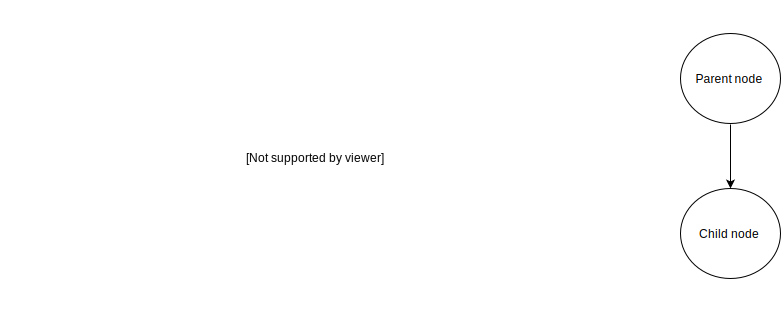
\includegraphics[width=1\linewidth]{figs/fig-json} \caption[_Figure 2._ An example of how two nodes might be described and stored in the blockchain and a depiction of how these two entries relate]{_Figure 2._ An example of how two nodes might be described and stored in the blockchain and a depiction of how these two entries relate.}\label{fig:fig_json}
\end{figure}

The nodes also include ``time-deposit'' and ``time-available'' entries;
these indicate the time-related aspects of the node. To ensure
chronology, the time the node is deposited into the ledger is included,
ensuring that if used as a parent, it precedes the child node.
Additionally, it makes sense that not all information can be made
available at the same time as the deposit takes place, which is why
``time-available'' is included to make clear when that information will
become available. There are various ways in which this time-locked
system could be implemented. Either the author can bear the
responsibility to deposit the materials in a timely manner, or a trusted
third-party can provide a service to automatically deposit these
materials. Alternatively, files could be encrypted and deposited at the
same time as the entry to the ledger is made, where the private key
needed to decrypt the files could be provided at the ``time-available''.
A system that incorporates ``time-available'' moves the discussion of
whether materials should be shared at all to when they can be shared
(i.e., not much can be justified to stay unavailable into perpetuity).

In order to provide identification and accountability of nodes, author
ORCIDs can be combined into unique author combinations, which also
diminishes gender and status bias during initial assessment (amongst
other things). These combinations can be created based on so-called
hashes (e.g., SHA256SUM with salting). For example, my ORCID is
\href{http://orcid.org/0000-0003-1050-6809}{\texttt{0000-0003-1050-6809}}
and that of one of my supervisors is
\href{http://orcid.org/0000-0003-2415-2933}{\texttt{0000-0003-2415-2933}}.
If I am the sole author, my ``authors'' hash would be
\texttt{a63d529d09b7c9de10e2e9cd71d51acec2f33f4f01af09eda5da152e0730f33f},
but if I am first author and my supervisor is second author, the hash is
different (i.e.,
\texttt{494a82a472b301e95a08b9334fc962a03f7cb196c72c10d997e75cf0d5c00de7}).
If we do not disclose these hashes or that we authored these nodes in
some composition, it is practically impossible to reverse the hash into
the identifiable ORCIDs. These hashes are not meant as a foolproof way
to safeguard author identity and remove biases in an absolute manner;
these hashes are primarily meant as a way to reduce the size of each
entry in the ledger (i.e., the hash is of the same length regardless of
how many authors are included) and to obfuscate the author's identity.
Such obfuscation is helpful to reduce bias in peer assessments.

What types of nodes are contained in the ledger is up for discussion.
For example, it is relatively clear that there can be ``theory'',
``hypothesis'', ``methods'', ``data'', ``analysis'', ``results'', and
``discussion'' nodes to cover the largest part of empirical research.
However, there are various other types of nodes that will not fit into
this rather restrictive taxonomy (e.g., ``opinion'' or those related to
qualitative research). Moreover, over time, new types of nodes might be
the result of natural development in scholarly research (e.g., due to
additions or changes to the scientific method). As such, the system
needs to be dynamic about the types of nodes it can include, but there
should also not be total chaos in the types of nodes. This node taxonomy
will require empirical study within the scholarly community to provide
an evidence-base for an initial version.

The contents of each node can vary, depending on the type of node. For
example, one node can refer to just one file directly (e.g., a
\texttt{csv} dataset), whereas others can refer to entire folders,
containing sets of files. For example, a data node can contain multiple
data files if it refers to a folder, or a theory section can contain the
text in various (open) formats, such as Markdown and XML. Moreover,
nodes on p2p networks such as \texttt{dat} by default support large
files (e.g., 50GB); such large file storage is becoming increasingly
necessary with the large amount of data available.

In order to deposit nodes onto the ledger, the depositor needs to agree
that the contents are licensed CC 0, in order to maximize legal
certainty regarding reuse of the contents. The current copyright system
has created the problem of inaccessibility and CC 0 empowers access by
default. Moreover, restrictive licensing also comes with duties to
enforce the license, if it is to mean anything to begin with. Enforcing
a restrictive license requires scholars to legally pursue those who
infringe their copyrights, detracting from their research time. As such,
scholars are not the ones who benefit from restrictive licensing, and
neither does the scholarly community at large.

\chapter{Conclusion}\label{conclusion}

At OpenCon2016, Brewster Kahle mentioned that the scholarly system
should be ``locked open''. After this talk I spent much time thinking
about how this could be done. Using a decentralized and distributed
system, as I tried to conceptualize throughout this article, is my
initial attempt at realizing a ``locked open'' system that benefits not
just the scholarly community, but also those that aim to generate value
from these outputs. By shifting from a knowledge commodification to a
commodification of how that knowledge is consumed, free access and reuse
becomes beneficial to all parties. This is key to create a sustainable
eco-system where scholars and companies can cooperate instead of
compete, as we currently do.

\section{References}\label{references}

\bibliography{library.bib}



\end{document}
